\documentclass[15pt]{beamer}
\usepackage[frenchb]{babel}
\usepackage[utf8]{inputenc}
\usepackage[T1]{fontenc}

% ----- rearranged from https://tex.stackexchange.com/questions/83882/how-to-highlight-
%                  python-syntax-in-latex-listings-lstinputlistings-command#83883 

% Default fixed font does not support bold face
\DeclareFixedFont{\ttb}{T1}{txtt}{bx}{n}{12} % for bold
\DeclareFixedFont{\ttm}{T1}{txtt}{m}{n}{12}  % for normal

% Custom colors
\usepackage{color}
\definecolor{deepblue}{rgb}{0,0,0.5}
\definecolor{deepred}{rgb}{0.6,0,0}
\definecolor{deepgreen}{rgb}{0,0.5,0}

\usepackage{listings}
\lstset{escapeinside={<@}{@>}}

%
% ------- PYTHON -------  
%

% Python style for highlighting
\newcommand\pythonstyle{\lstset{
language=Python,
xleftmargin=0cm,
numbersep = 0.5cm,
numbers=left, 
numberstyle=\tiny\bf, 
stepnumber=5, 
basicstyle=\ttm,
otherkeywords={self, echo, cat, mv, cp},             % Add keywords here
keywordstyle=\ttb\color{deepblue},
emph={MyClass,__init__},          % Custom highlighting
emphstyle=\ttb\color{deepred},    % Custom highlighting style
stringstyle=\color{deepgreen},
frame=tb,                         % Any extra options here (tb)
showstringspaces=false            % 
}}


% Python environment
\lstnewenvironment{python}[1][]
{
\pythonstyle
\lstset{#1}
}
{}

% Python for external files
\newcommand\pythonexternal[2][]{{
\pythonstyle
\lstinputlisting[#1]{#2}}}

% Python for inline
\newcommand\pythoninline[1]{{\pythonstyle\lstinline!#1!}}

%
% -------  C  -------  
%

% C style for highlighting
\newcommand\Cstyle{\lstset{
language=C,
xleftmargin=0cm,
numbersep = 0.5cm,
numbers=left, 
numberstyle=\tiny\bf, 
stepnumber=5, 
basicstyle=\ttm,
otherkeywords={sizeof},             % Add keywords here
keywordstyle=\ttb\color{deepblue},
emph={MyClass,__init__},          % Custom highlighting
emphstyle=\ttb\color{deepred},    % Custom highlighting style
stringstyle=\color{deepgreen},
frame=tb,                         % Any extra options here
showstringspaces=false            %
}}


% C environment
\lstnewenvironment{C}[1][]
{
\Cstyle
\lstset{#1}
}
{}

% C for external files
\newcommand\Cexternal[2][]{{
\Cstyle
\lstinputlisting[#1]{#2}}}

% C for inline
\newcommand\Cinline[1]{{\Cstyle\lstinline!#1!}}

%
% -------  ASSEMBLER -------  
%

% Assembler style for highlighting
\newcommand\assemblerstyle{\lstset{
language=[x86masm]Assembler,
xleftmargin=0cm,
numbersep = 0.5cm,
numbers=left, 
stepnumber=5, 
numberstyle=\tiny\bf, 
basicstyle=\ttm,
otherkeywords={sizeof},             % Add keywords here
keywordstyle=\ttb\color{deepblue},
emph={MyClass,__init__},          % Custom highlighting
emphstyle=\ttb\color{deepred},    % Custom highlighting style
stringstyle=\color{deepgreen},
frame=tb,                         % Any extra options here
showstringspaces=false            % 
}}


% assembler environment
\lstnewenvironment{Assembler}[1][]
{
\assemblerstyle
\lstset{#1}
}
{}

% assembler for external files
\newcommand\assemblerexternal[2][]{{
\assemblerstyle
\lstinputlisting[#1]{#2}}}

% assembler for inline
\newcommand\assemblerinline[1]{{\assemblerstyle\lstinline!#1!}}

%
% -------  BASH -------  
%

% Bash style for highlighting
\newcommand\bashstyle{\lstset{
language=Bash,
xleftmargin=0cm,
numbersep = 0.5cm,
numbers=left, 
numberstyle=\tiny\bf, 
stepnumber=5, 
basicstyle=\ttm,
otherkeywords={self, echo, cat, mv, cp},             % Add keywords here
keywordstyle=\ttb\color{deepblue},
emph={MyClass,__init__},          % Custom highlighting
emphstyle=\ttb\color{deepred},    % Custom highlighting style
stringstyle=\color{deepgreen},
frame=tb,                         % Any extra options here (tb)
showstringspaces=false            % 
}}


% Bash environment
\lstnewenvironment{bash}[1][]
{
\bashstyle
\lstset{#1}
}
{}

% Bash for external files
\newcommand\bashexternal[2][]{{
\bashstyle
\lstinputlisting[#1]{#2}}}

% Bash for inline
\newcommand\bashinline[1]{{\bashstyle\lstinline!#1!}}
 % where are all the options about syntax highlight.
% Common commands 
\newcommand{\stdin}{\bashinline{stdin} }
\newcommand{\stdout}{\bashinline{stdout} }
\newcommand{\stderr}{\bashinline{stderr} }
\newcommand{\SubBytes}{\text{\Cinline{SubBytes}~}}
\newcommand{\Sub}{\text{\Cinline{Sub}~}}
\newcommand{\AddRoundKey}{\text{\Cinline{AddRoundKey}~}}
\newcommand{\ShiftRows}{\text{\Cinline{ShiftRows}~}}
\newcommand{\MixColumns}{\text{\Cinline{MixColumns}~}}
\newcommand{\Mix}{\text{\Cinline{Mix}~}}
\newcommand{\shiftkey}{\text{\Cinline{shift\_key}~}}
\newcommand{\key}{\text{\Cinline{key}~}}
\newcommand{\state}{\text{\Cinline{state}~}}
\newcommand{\xor}{\:\oplus\:}

\newcommand{\byte}{\Cinline{byte}}
\newcommand{\word}{\Cinline{word}}
\newcommand{\nibble}{\Cinline{nibble}}

\usepackage{ulem}
\usepackage{graphicx}
\usepackage{xcolor}
%\usetheme{theme/beamerthememetropolis}
\usepackage{beamerthememetropolis}

% \usepackage{parallel}
\usepackage{tikz}
\usetikzlibrary{positioning}
\usetikzlibrary{calc}
\usetikzlibrary{decorations.pathreplacing}

\usepackage{xcolor} % to put colors in equations, ex:  \color{red} ...  or
% \textcolor{red}{foo}: \

\usepackage{wrapfig}

\usepackage{enumerate}

\title{Les FHE, c'est facheux.}
\date{\today}
\author{Lucas Roux \& Eric Sageloli}

\begin{document}

% ------------------------------------------------------------------------------------------------

\begin{frame}
  \maketitle
\end{frame}

% ------------------------------------------------------------------------------------------------

\begin{frame}
  \frametitle{Introduction : contexte Whitebox}
\begin{itemize}
  \item Contexte classique:  blackbox
  \item DRM 
  \item nouveau contexte : whitebox
  \end{itemize}
\end{frame}

% ------------------------------------------------------------------------------------------------

\begin{frame}
  
  \frametitle{Introduction : comment faire un oral ?}
  
  
  Première idée : 
  
  \begin{columns}[T] % align columns
    
    \begin{column}{.48\textwidth}
      \begin{figure}
        \begin{center}
          \begin{tikzpicture}[scale = 1, transform shape]
	    \node[inner sep=0pt] (alice) at (0,0)
    {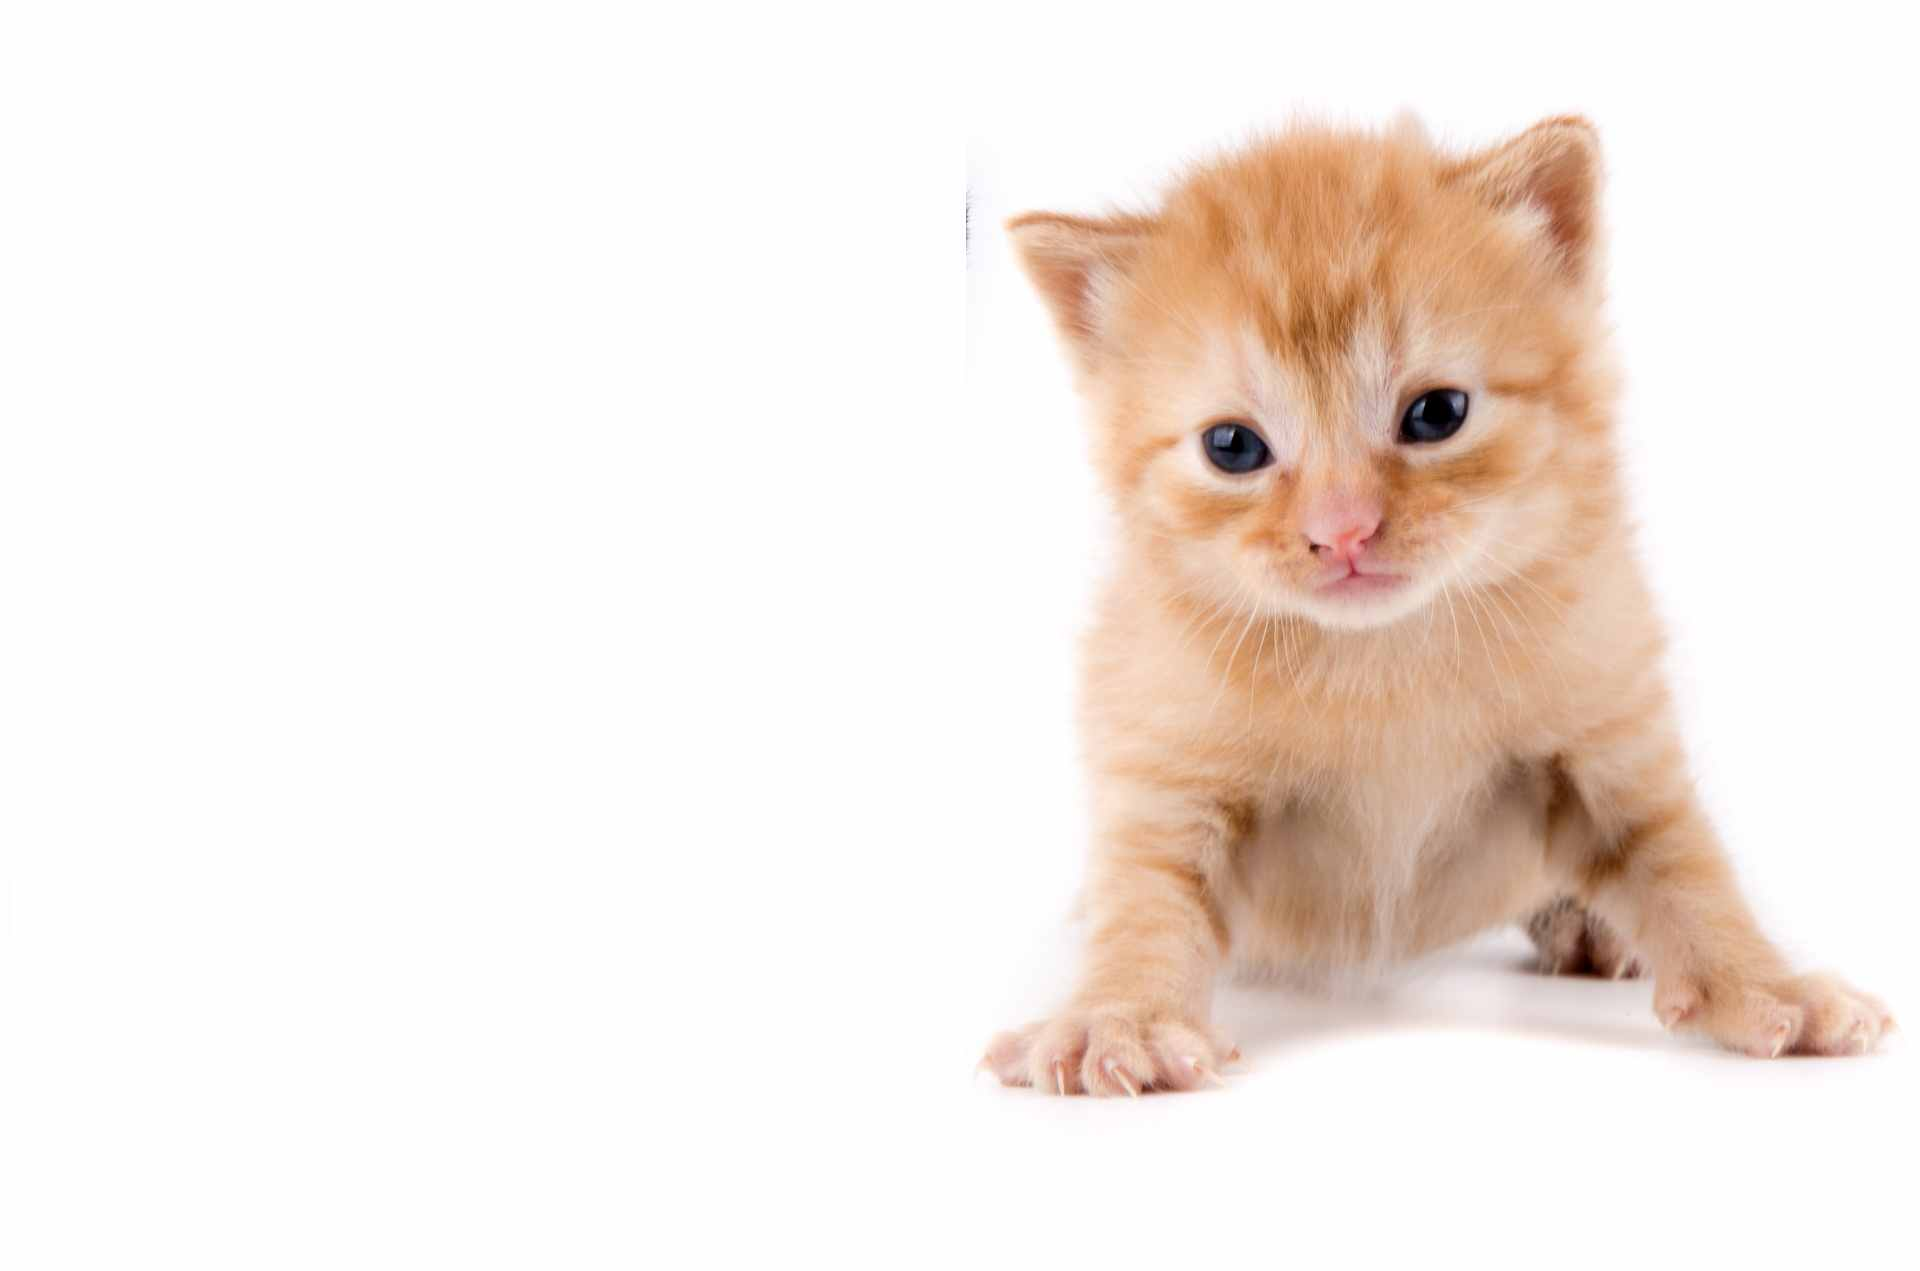
\includegraphics[width=.25\textwidth]{../pictures/examples/alice.jpeg}};
\node[inner sep=0pt] (bob) at ($(alice) + (6,0)$)
    {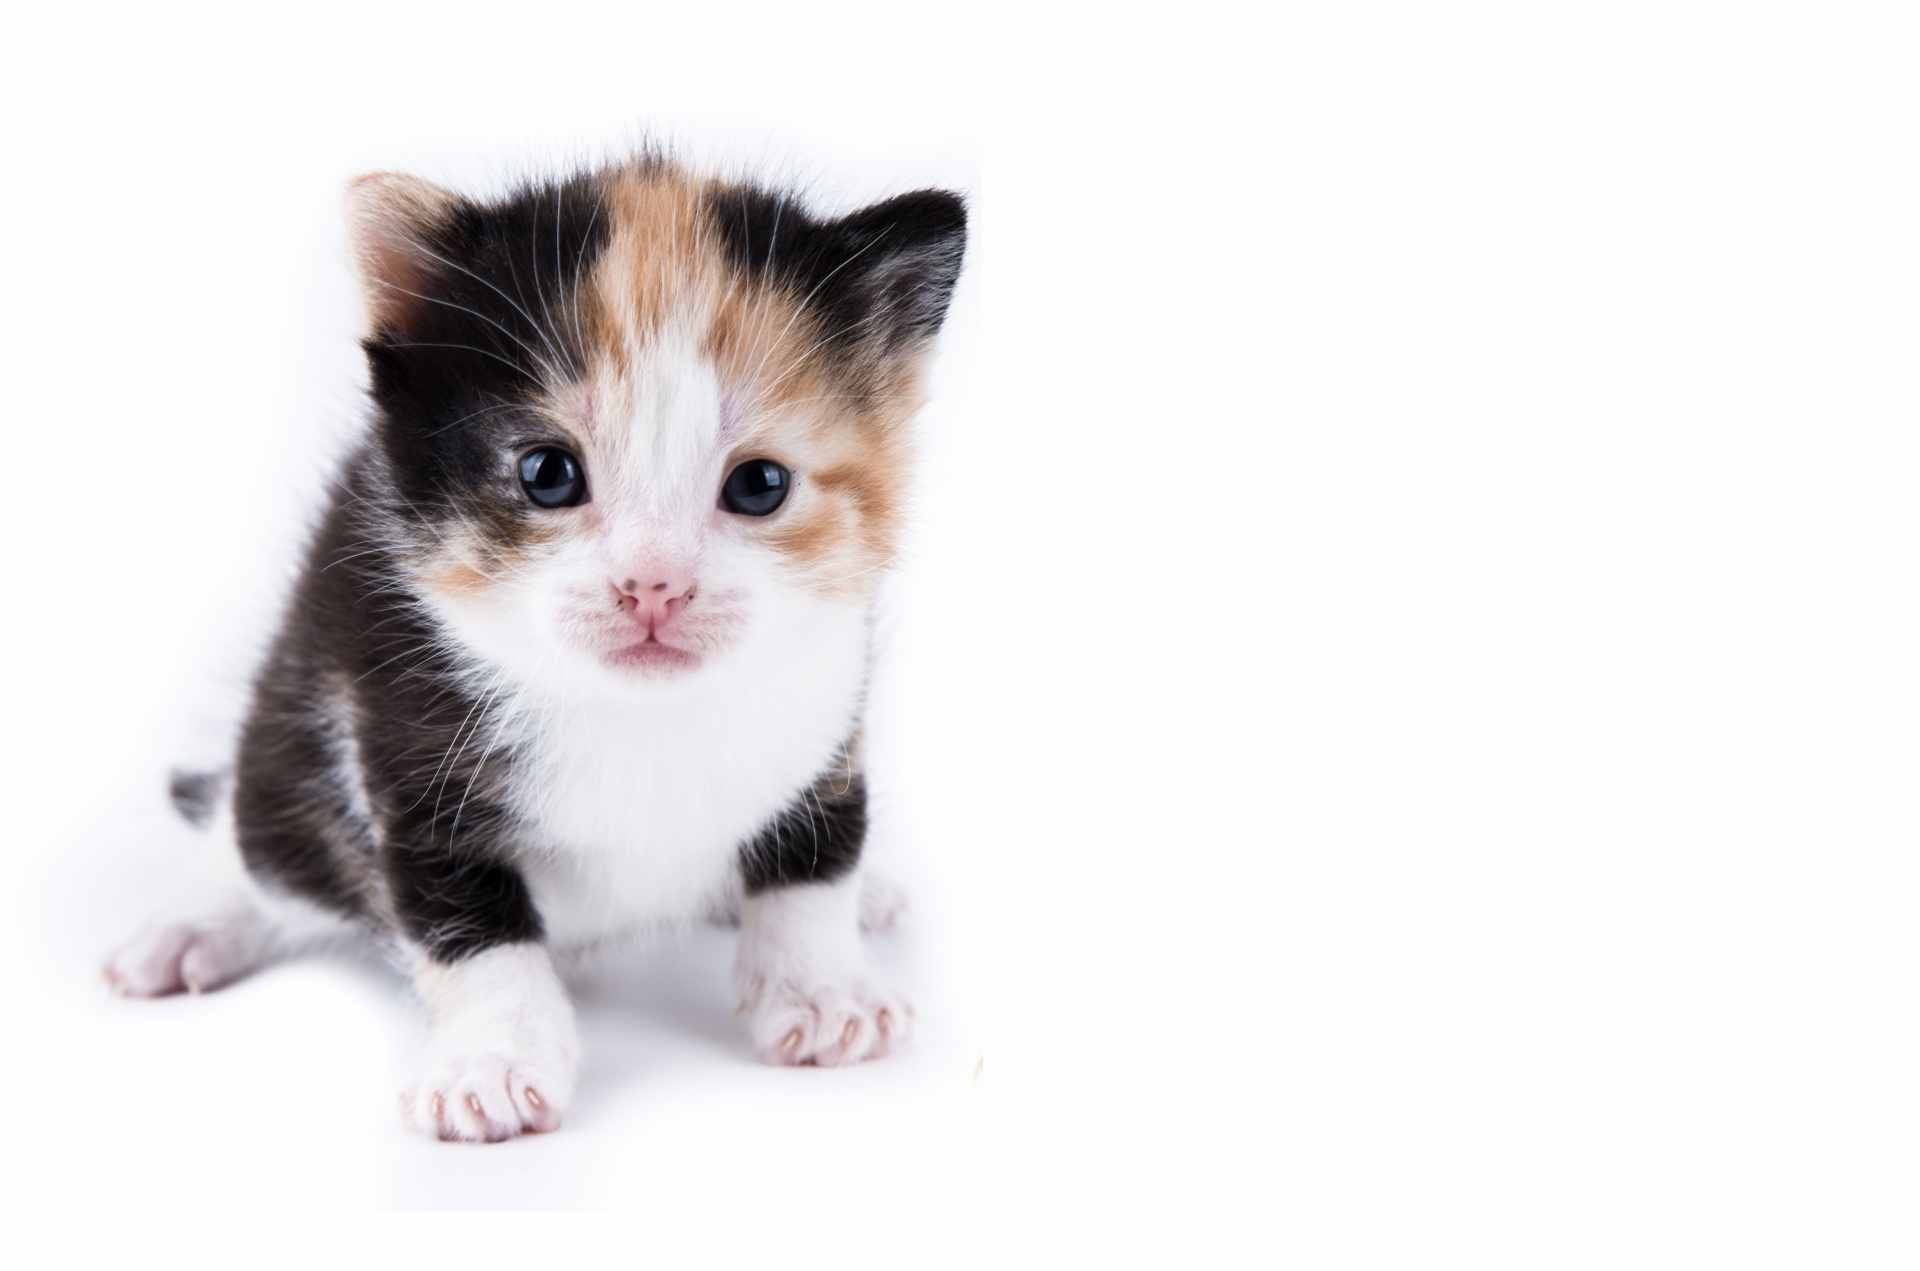
\includegraphics[width=.25\textwidth]{../pictures/examples/bob.jpeg}};
\node[inner sep=0pt] (eve) at ($(alice) + (3,2)$)
    {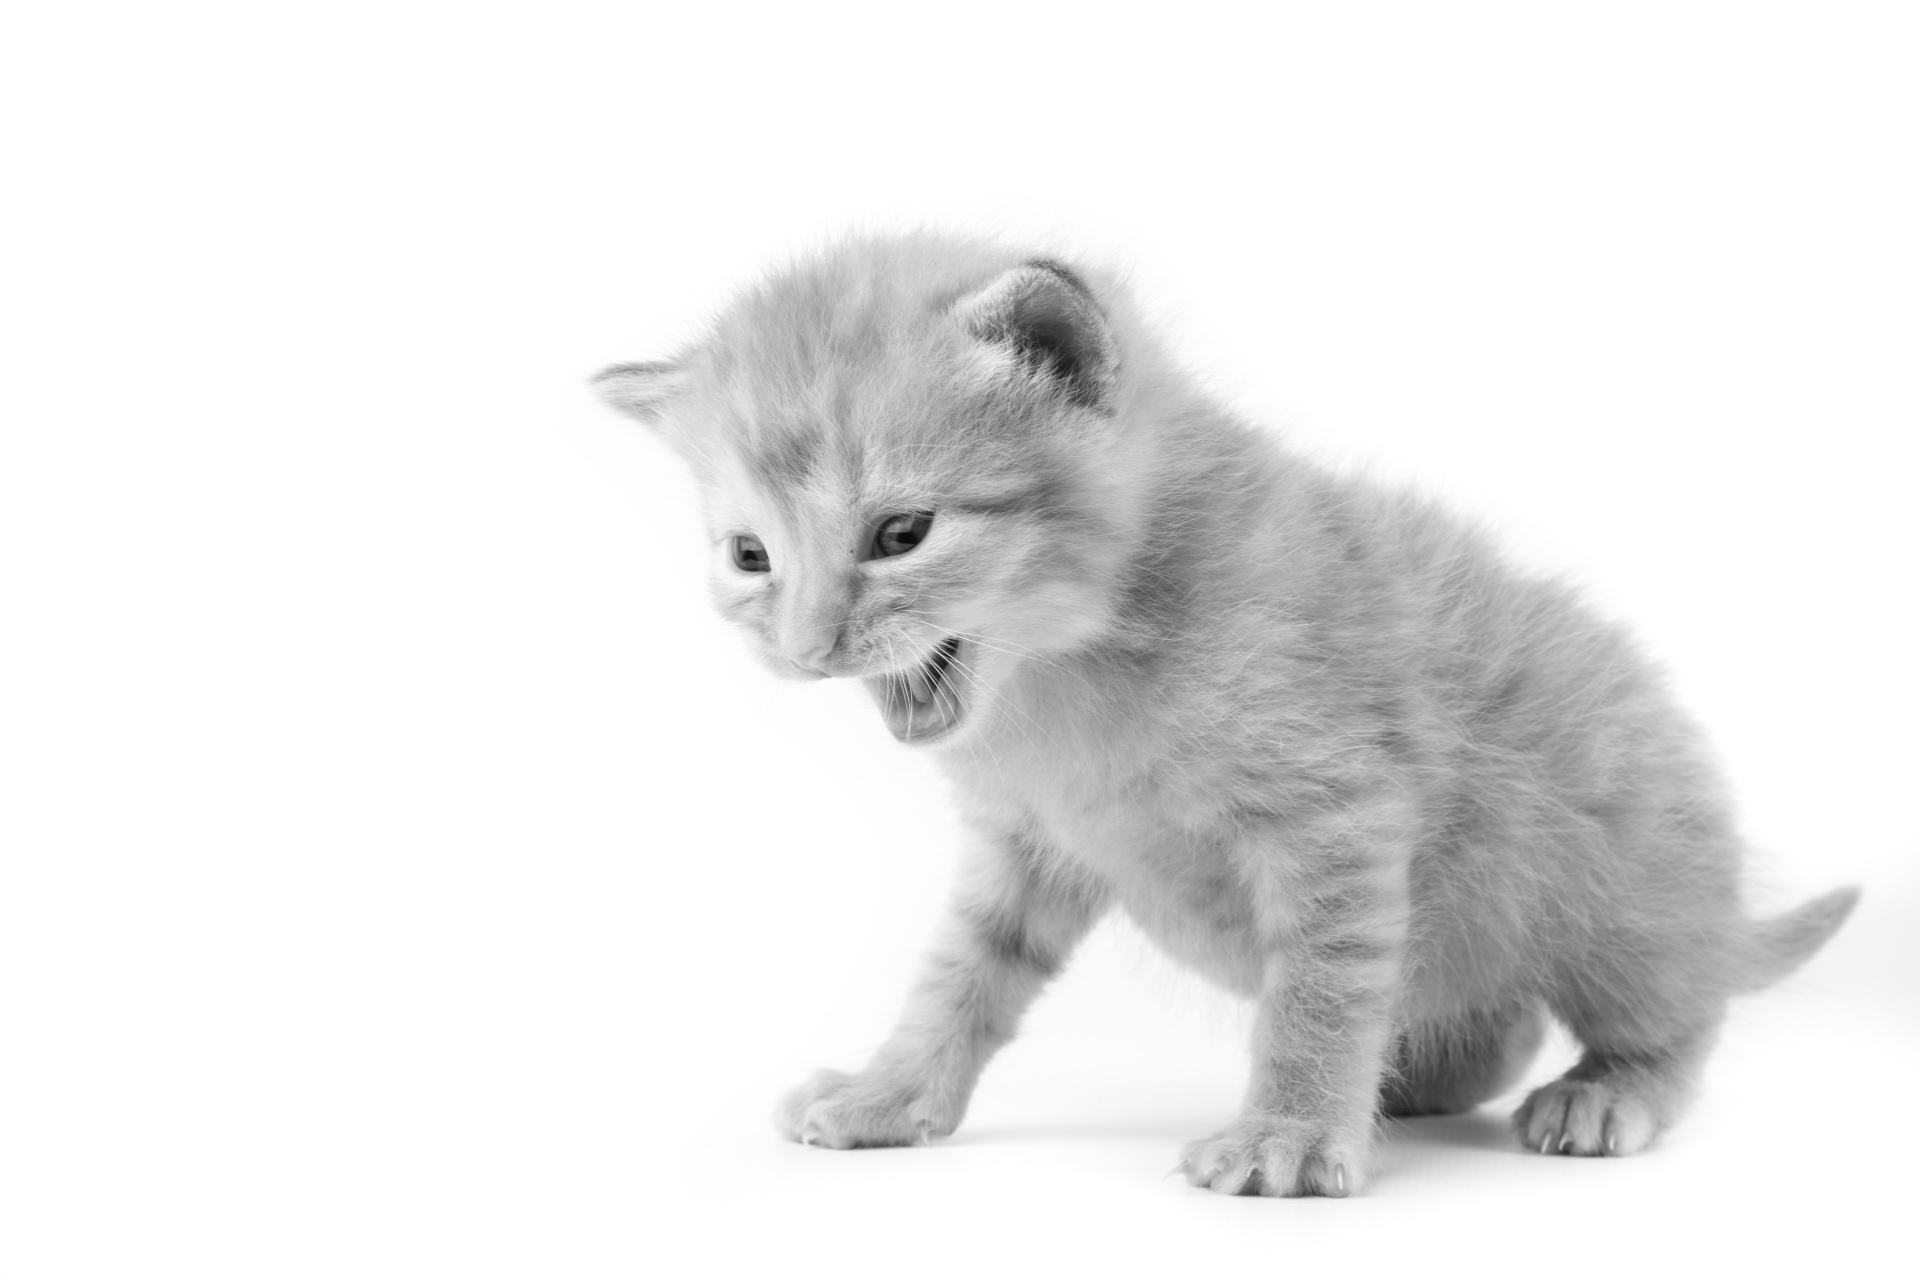
\includegraphics[width=.25\textwidth]{../pictures/examples/eve.jpg}};
\node[inner sep=0pt] (alicec) at ($(alice) + (-1,0)$)
    {
\includegraphics[width=.10\textwidth]{../pictures/examples/computer.jpg}};
\node[inner sep=0pt] (bobc) at ($(bob) + (1,0)$)
    {
\includegraphics[width=.10\textwidth]{../pictures/examples/computer.jpg}};
\node  at ($(bob) + (1.2,-1)$)
    {\tiny déchiffrement\_AES.c};
\node at ($(alice) + (-1,-1)$)
{\tiny chiffrement\_AES.c};

\node[color = red] at ($(alice) + (-1,0.2)$) {M};
\node[color = red] at ($(bob) + (1,0.2)$) {\tiny $E_k(M)$};

\node[color = red] (C) at ($(alice) + (3,0.5)$) {\small$E_k(M)$};

\draw[->, thick] (alice) -- (bob);

          \end{tikzpicture}
        \end{center}
      \end{figure}
    \end{column}

    \begin{column}{.48\textwidth}
      \vspace{2cm}
      \begin{itemize}
      \item<2-> Et pourquoi pas?;
      \item<3-> Ehehe
        \begin{itemize}
        \item $2^{128}$ entrées
        \item 16 octets par sortie
        \item $16 * 2^{128} = 2^{132}$ octets 
        \end{itemize}
      \end{itemize}
    \end{column}
    
  \end{columns}

\end{frame}

% ------------------------------------------------------------------------------------------------

\begin{frame}
  \frametitle{Introduction : comment cacher la clé ?}
  \begin{figure}
    \begin{center}
      \begin{tikzpicture}[scale = 0.6, transform shape]
    {
\includegraphics[width=.10\textwidth]{../pictures/examples/computer.jpg}};
      \end{tikzpicture}
    \end{center}
  \end{figure}

  Pour chaque table :
  \begin{itemize}
  \item $2^8$ entrées
  \item 1 octet en sortie
  \item taille : $2^8$ octets
  \end{itemize}

  taille totale : $16 * 2^8 = 2^{12}$ octet = 4 Ko

  \pause
  \vspace{0.7cm}

  \begin{itemize}
  \item La clé n'est plus complètement obfusquée.
  \item<2->On aura besoin de $2032$ tables, stockés sur $500KB$
  \end{itemize}
\end{frame}

\end{document}
